\chapter{Houston Interviews: Income, Assets, Access, and Leverage}

This chapter follows a School of Hard Knocks entrepreneurship interview, curated for the LazyEarn track by LazyingArt LLC. The video is not a blackboard lecture; it is a sequence of street interviews in Houston. The mathematical work, therefore, is not formal physics or operator algebra. It is careful bookkeeping: separating income from assets, salary from ownership, risk from upside, and anecdote from mechanism. We will preserve the order of the interview and use simple quantitative notation only where it clarifies what the speakers actually claim.

\section{Houston as a Field Test of Wealth Claims}

The opening is deliberately fast. Before we are given a method, we hear outcomes: a portfolio ``about $420 million,'' a multi-billion-dollar insurance brokerage firm, industrial real estate, champagne, and a Lamborghini. The host then frames Houston as a city with many millionaires and sets the task: ask people how they became wealthy.

The first thing we should do is not believe or disbelieve the numbers. We should classify them. A number can mean annual income, portfolio value, realized gain, business valuation, salary, or tax benefit. These are different objects.

Let us introduce notation for the basic distinction:
\begin{align}
Y &:= \hbox{annual earned income or salary},\\
S &:= \hbox{annual savings},\\
P &:= \hbox{portfolio value},\\
I &:= \hbox{initial investment},\\
V &:= \hbox{claimed investment or portfolio outcome}.
\end{align}

The interview repeatedly moves between these objects. If we do not keep them separate, the chapter becomes a pile of impressive numbers. If we keep them separate, the chapter becomes a map of wealth mechanisms.

\begin{figure}
\centering
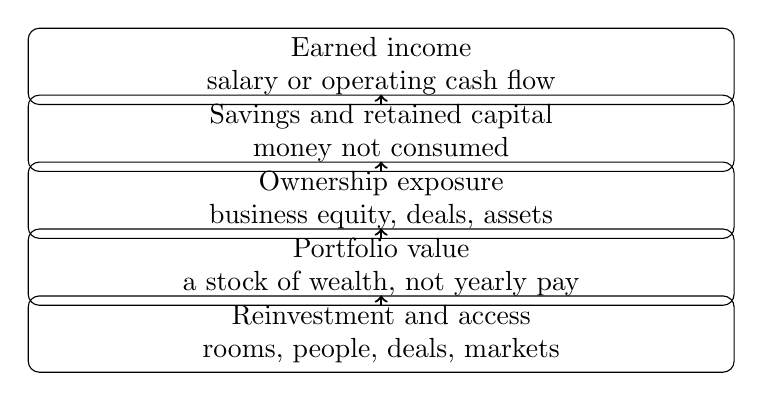
\begin{tikzpicture}[
  node distance=0.85cm,
  every node/.style={draw, rounded corners, align=center, text width=0.72\linewidth, minimum height=0.75cm},
  arrow/.style={->, thick}
]
\node (income) {Earned income\\salary or operating cash flow};
\node (saving) [below of=income] {Savings and retained capital\\money not consumed};
\node (ownership) [below of=saving] {Ownership exposure\\business equity, deals, assets};
\node (portfolio) [below of=ownership] {Portfolio value\\a stock of wealth, not yearly pay};
\node (access) [below of=portfolio] {Reinvestment and access\\rooms, people, deals, markets};
\draw[arrow] (income) -- (saving);
\draw[arrow] (saving) -- (ownership);
\draw[arrow] (ownership) -- (portfolio);
\draw[arrow] (portfolio) -- (access);
\end{tikzpicture}
\caption{A transcript-derived reconstruction of the main wealth pathway in the Houston interviews. It is not a screenshot or board diagram; it is a compact way to distinguish income, savings, ownership, portfolio value, and access.}
\end{figure}

\section{Foundation Before Speed}

The first full interview slows the montage down. The speaker says he runs a company, solves problems, and now leads an insurance brokerage firm described as a multi-billion-dollar company. The emphasis is not on a trick. It is on leadership, people, education, and patience.

When asked what he would tell his younger self, he gives two ideas that belong together. First, be bold. Second, get foundation. He tells young people to spend four or five years understanding their discipline before going out on their own. In other words, the first mechanism is not leverage; it is competence.

Then the interview turns to personal finance. The speaker recommends reading \emph{The Wealthy Barber} and \emph{The Millionaire Next Door}, then saving early. The usable claim in the transcript is clear even though the phrase ``rule of seven'' is ambiguous: save 10 to 20 percent.

We can write the savings relation as
\begin{equation}
S=sY,
\end{equation}
where \(s\) is the savings rate. The transcript-backed range is
\begin{equation}
s\in[0.10,0.20].
\end{equation}
For the salary range explicitly mentioned in the interview,
\begin{equation}
Y\approx \$70{,}000 \hbox{ to } \$80{,}000.
\end{equation}
So the corresponding annual savings range is
\begin{align}
S_{\min} &=0.10(\$70{,}000)=\$7{,}000,\\
S_{\max} &=0.20(\$80{,}000)=\$16{,}000.
\end{align}

This does not prove that everyone who saves this amount becomes a millionaire by a certain age. The speaker makes that claim as interview advice. What the arithmetic does show is the mechanism: savings converts earned income into capital that can later be deployed.

\subsection{Question \& Answer}

\paragraph{Question.}
Can ordinary earned income become wealth, or does wealth require ownership leverage?

\paragraph{Answer.}
The first interview says ordinary income can begin the process if it is paired with discipline: save early, learn a field, and build a foundation. But the later interviews show why saving alone is not the whole story. Savings creates capital; ownership decides whether that capital remains small, compounds slowly, or gains exposure to much larger outcomes.

\section{Portfolio Value Is Not Annual Income}

The next major interview shifts the scale. The speaker describes starting in oil and gas as a project manager after attending TCU and Rice University. From project management, he says he became an angel investor, had successful exits, and then started his own private equity firm.

The host asks the same opening question from the montage: what is the most money you ever made in a single year? The answer is important because the speaker corrects the frame. He says it is not really based on dividends or what he makes from companies. It is more about what he has as far as portfolio value. Then he gives the portfolio range: about $420 million.

In notation, the interview claim is
\begin{equation}
P\approx \$420{,}000{,}000.
\end{equation}
But \(P\) is not \(Y\). Portfolio value is a stock of wealth. Annual income is a flow. Dividends are a flow. Realized sale proceeds are a different flow. A large portfolio can produce small annual cash income, or large income, depending on liquidity, distributions, taxes, leverage, and valuation.

\subsection{Question \& Answer}

\paragraph{Question.}
When someone says he made or has ``$420 million,'' what exactly is being measured?

\paragraph{Answer.}
In this interview, the speaker himself points away from ordinary annual income. He describes the number as a portfolio range, not as salary and not as dividends. The notes should therefore treat \(P\approx \$420\) million as an interview claim about portfolio value. It should not be rewritten as yearly cash income.

\section{Risk, Asymmetry, and Access}

The host then asks for the biggest risk. The answer is Snapchat. The speaker says Snapchat was raising a seed round in 2010, and that he invested a large amount relative to his situation at the time. He says his salary was $80,000 and someone was asking for $20,000 out of pocket.

The simplest useful calculation is exposure:
\begin{equation}
E=\frac{I}{Y}.
\end{equation}
With the transcript's numbers,
\begin{equation}
E=\frac{\$20{,}000}{\$80{,}000}=0.25.
\end{equation}
So the risk was not merely that $20,000 is a large number. It was large relative to the salary base: one quarter of a year's salary.

\paragraph{Worked exposure calculation.}
\begin{enumerate}
\item Start from the annual salary claim, \(Y=\$80{,}000\).
\item Start from the investment claim, \(I=\$20{,}000\).
\item Divide investment by annual salary:
\[
E=\frac{I}{Y}.
\]
\item Substitute the transcript values:
\[
E=\frac{20{,}000}{80{,}000}=0.25.
\]
\item Interpret the result as concentrated exposure: the investment represented 25 percent of one year's salary.
\end{enumerate}

The speaker later claims a result of about $72 million from Snap and other companies in his portfolio. We should be precise here. The transcript does not cleanly say that \(V=\$72\) million came only from the $20,000 Snapchat investment. It says Snap and all the other companies in the portfolio.

A general return multiple can be defined as
\begin{equation}
M=\frac{V}{I}.
\end{equation}
But in this case the clean multiple is uncertain because \(V\) mixes Snap with other portfolio companies. The right lesson is asymmetry, not a verified formula. A finite investment can be lost, but ownership in a very successful company can create upside far beyond the original salary scale.

The speaker then gives a different kind of answer: marketing. Asked what takes a business from seven to eight and eventually nine figures, he says marketing. The host's recap turns that into a network thesis: to find companies, deals, and rooms, he says, the investor had to work with people who were wealthier and better connected.

That is the bridge from risk to access. Capital matters, but access determines which risks are even available.

\section{Operations: Showing Up, Details, and Listening}

After the portfolio story, the lecture returns to operating businesses. This is a necessary change in rhythm. If we only keep the angel-investment story, we miss the ordinary disciplines that make businesses credible enough to attract capital or customers.

A restaurant operator gives the simplest operating principle: 90 percent of success is showing up. He explains that showing up means people trust you. They know you will be there like clockwork. The point is not glamorous, but it is structural. Reliability converts time into trust.

We can write a narrow operating chain:
\begin{equation}
\hbox{repeated presence}\longrightarrow
\hbox{trust}\longrightarrow
\hbox{opportunity}.
\end{equation}
This is not a law of nature. It is the mechanism the speaker describes.

The same operator then talks about details: remembering children's names, birthday cakes, surprises, handwritten letters, and thank-you notes. These are small actions, but they differentiate the restaurant from competitors. The business claim is that customer memory and care become a moat.

Later, an industrial real estate speaker gives a parallel operating lesson. He says his company buys or builds and leases large industrial properties across the country. He claims over a million dollars in a single year and says the secret to scaling is working 60 hours a week:
\begin{equation}
H\approx 60\ \hbox{hours/week}.
\end{equation}
When asked about sales, he says the best way to close deals is to listen. The reason is practical: if we do not understand needs and wants, we cannot fulfill them. This converts sales from pressure into diagnosis.

\section{Marketing, Relationships, and Brand Formation}

The marketing motif appears first in the private equity interview: marketing takes a company from seven figures to eight and eventually nine. It appears again in the renewable-energy social media marketer, who says the secret to marketing and building a strong brand is networking and building relationships outside social media platforms.

That is a useful correction. Marketing is not only posting. In these interviews, marketing means distribution, reputation, and relationship density. A brand gets stronger when more people know what it stands for, trust the person behind it, and can repeat the value proposition.

The champagne founder closes the loop. He says he set out to redefine champagne. He describes a long history: restaurant industry, oil and gas, travel, wine regions, terroirs, and turning passion into a business case. His sales explanation is twofold: relationships and a product that is second to none. He contrasts this with conglomerates hiding behind large labels.

Here the transcript gives the most explicit product-market discipline. He advises founders to research the market, competitors, price point, premium positioning, margins, and contingencies. The clean bookkeeping relation for margins is
\begin{equation}
\hbox{gross margin}
=
\frac{\hbox{price}-\hbox{unit cost}}{\hbox{price}}.
\end{equation}
The point is not that the interview gives a spreadsheet. It does not. The point is that a premium product must be priced and costed deliberately. If costs come out higher than expected, the margin vanishes unless the founder built in contingency.

\begin{table}
\centering
\begin{tabular}{p{0.24\linewidth}p{0.25\linewidth}p{0.25\linewidth}p{0.17\linewidth}}
\hline
Interview context & Concrete claim & Mechanism & Caution\\
\hline
Insurance brokerage & Multi-billion-dollar company & Leadership, people, foundation & Claimed valuation scale\\
Savings advice & Save 10--20 percent & Convert income into capital & Not a guarantee\\
Angel investing & $20k risk on $80k salary & Ownership asymmetry & Outcome mixed with portfolio\\
Restaurant & Show up and remember details & Trust and differentiation & Local operating claim\\
Industrial real estate & 60 hours/week and listening & Work volume and diagnosis & Not universal formula\\
Champagne & Research price, market, margins & Premium positioning & Costs may exceed plan\\
\hline
\end{tabular}
\caption{A compact separation of anecdote, claim, mechanism, and caution from the transcript.}
\end{table}

\section{Real Estate, Tax Caveats, and Asset Structure}

The transcript returns several times to real estate. One speaker works in industrial real estate, buying or building and leasing large properties. Another mentions real estate investment trusts and a $1.2 million deal. The transcript also includes claims about tax breaks, caveats, nuances, buying assets under entities, leasing assets to oneself, and write-offs.

This material should be preserved, but cautiously. It is legally and financially sensitive, and parts of the transcript are garbled. We can still extract the conceptual distinction:
\begin{equation}
\hbox{asset return}
\neq
\hbox{tax effect}
\neq
\hbox{cash income}.
\end{equation}
A business owner may care about all three, but they are not the same number. The interview claims that structures, entities, and tax treatment can affect how wealth is preserved. These notes should not turn that into tax advice. The usable lesson is that advanced business ownership requires understanding structure, not just buying an asset.

\subsection{Question \& Answer}

\paragraph{Question.}
Are tax breaks and entity structures the wealth mechanism, or are they secondary?

\paragraph{Answer.}
In this transcript, they are secondary but important. The primary mechanisms are ownership, cash flow, deal access, operations, sales, and product-market discipline. Entity structure and tax treatment affect how gains are held, protected, or reinvested. Because the transcript is garbled in this section and the subject is technical, the chapter should treat these comments as prompts for professional advice, not as instructions.

\section{Repeated Leverage}

The chapter closes by assembling the pattern. No single interview gives the whole map. The insurance executive gives foundation, saving, and leadership. The investor gives ownership risk, portfolio value, marketing, and access. The restaurant owner gives showing up and details. The Lamborghini exchange gives belief and visualization, but the more concrete version is: visualize, act, and do not quit. The engineer gives decision quality and adaptability. Industrial real estate gives work volume and listening. Social media marketing gives relationships beyond platforms. The real estate and REIT discussion gives caveats around structure. The champagne founder gives research, margins, premium positioning, relationships, product quality, and contingencies.

The resulting model is not a promise. It is a sorting device:
\begin{align}
\hbox{wealth building}
&\approx
\hbox{discipline}
+\hbox{ownership}
+\hbox{asymmetry}
+\hbox{trust} \notag\\
&\quad
+\hbox{relationships}
+\hbox{research}
+\hbox{margin control}
+\hbox{judgment}.
\end{align}

That expression is not a formula to calculate net worth. It is a compact summary of the transcript's recurring mechanisms. The interviews show that wealth stories often begin with a visible result, but the useful work begins when we ask what kind of number we are hearing, what risk produced it, what operating behavior sustained it, and what relationships made it possible.